\documentclass[a4paper,UTF8,titlepage]{ctexart}
\def\pgfsysdriver{pgfsys-dvipdfmx.def}
\usepackage{tikz}
\pagestyle{plain}

\begin{document}
\title{exampe}
\maketitle

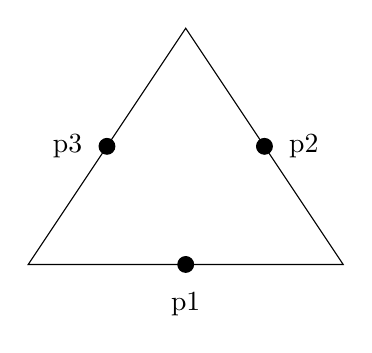
\begin{tikzpicture}
	\draw (0,0)--(4,0)--(2,3)--cycle;
	\filldraw (2,0)   circle(.1)
			  (3,1.5) circle(.1)
			  (1,1.5) circle(.1);
	\node at(2,-0.5)   {p1};
	\node at(3.5,1.5) {p2};
	\node at(0.5,1.5) {p3};
\end{tikzpicture}

\begin{figure}[h]
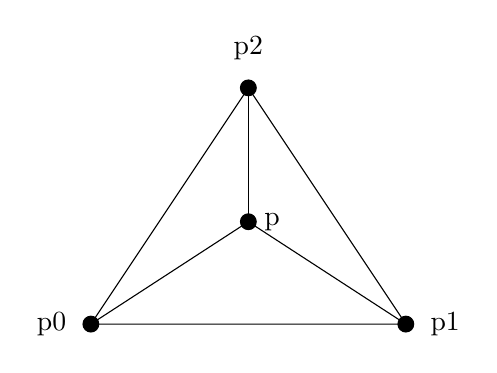
\begin{tikzpicture}
	\draw (0,0)--(4,0)--(2,3)--cycle;
	\draw (0,0)--(2,1.3)--(4,0);
	\draw (2,1.3)--(2,3);
	\filldraw (0,0)   circle(.1)
	          (4,0) circle(.1)
	          (2,3) circle(.1)
	          (2,1.3) circle(.1);
	\node at(-0.5,0)  {p0};
	\node at(4.5,0)   {p1};
	\node at(2,3.5)   {p2};
	\node at(2.3,1.3) {p};
\end{tikzpicture}
\caption{划分}
\label{1}
\end{figure}

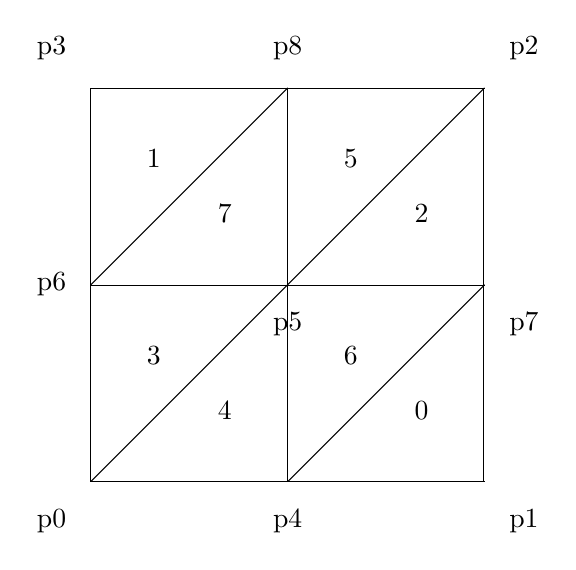
\begin{tikzpicture}
	\draw [step=71pt] (0,5) grid (5,0);
	\draw (0,0)--(5,5);
	\draw (0,2.5)--(2.5,5);
	\draw (2.5,0)--(5,2.5);
	
	\node at(-0.5,-0.5) {p0};
	\node at(2.5,-0.5)  {p4};
	\node at(5.5,-0.5)  {p1};
	\node at(-0.5,2.5)  {p6};
	\node at(2.5,2)     {p5};
	\node at(5.5,2)     {p7};
	\node at(-0.5,5.5)  {p3};
	\node at(2.5,5.5)   {p8};
	\node at(5.5,5.5)   {p2};
	
	\node at(0.8,1.6) {3};
	\node at(1.7,0.9) {4};
	\node at(3.3,1.6) {6};
	\node at(4.2,0.9) {0};
	\node at(0.8,4.1) {1};
	\node at(1.7,3.4) {7};
	\node at(3.3,4.1) {5};
	\node at(4.2,3.4) {2};
\end{tikzpicture}

\begin{figure}[h]
	\centering
	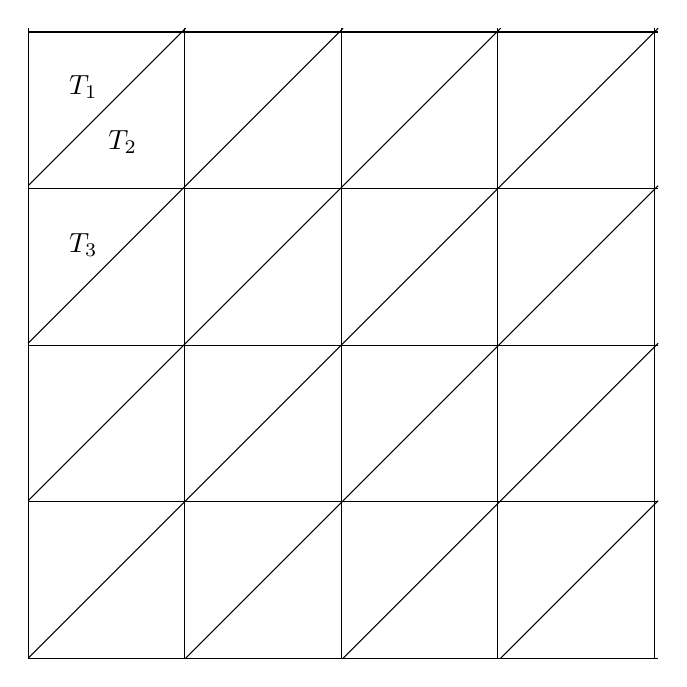
\begin{tikzpicture}
		\draw [step=56.56pt] (0,8) grid (8,0);
		
		\draw (0,6) -- (2,8);
		\draw (0,4) -- (4,8);
		\draw (0,2) -- (6,8);
		\draw (0,0) -- (8,8);
		\draw (2,0) -- (8,6);
		\draw (4,0) -- (8,4);
		\draw (6,0) -- (8,2); 
		
		\node at(0.7,7.25) {$T_1$};
		\node at(1.2,6.55) {$T_2$};
		\node at(0.7,5.25) {$T_3$};
	\end{tikzpicture}
\end{figure}

\end{document}